\chapter{Identification of drugs response properties and methods of tissue preparation for single cell measurements in patient derived xenografts %Establishing a transplant model and the methods for single cell dissociation 
}
\label{ch:Chapter 3}

\section{Motivation}
Single-cell whole genome sequencing and direct library prep (DLP) and RNA sequencing (scRNA-seq) are powerful tool for studying complex biological systems, such as tumor heterogeneity and tissue microenvironments. However, the sources of technical and biological variation in primary solid tumor tissues and patient-derived mouse xenografts for scRNA-seq are not well understood.
Due to the sensitivity of single-cell RNA sequencing (scRNA-seq), small changes in gene expression can dramatically influence the interpretation of biological data. scRNA-seq data is also subject to technical and biological noise \cite{potter2018single, stegle2015computational} Transcriptional machinery remains active at 37$^{\circ}$ °C, and extended incubation at high temperatures may introduce gene expression artifacts, independent of the biology at the time of harvest. Moreover, extended incubation at higher temperatures in the absence of nutrients or anchorage, or harsh dissociation, may induce apoptosis or anoikis, polluting the viable cell population or generating low-quality suspensions \cite{volovitz2016non}. Therefore, it is imperative to characterize the inherent variation and potential effects of cell isolation methods on the transcriptomic profiles of tissues. Recently, it has been shown that a serine protease (subtilisin A) isolated from a Himalayan glacier-resident bacterium, \textit{Bacillus lichenformis}, is suitable for dissociation of non-malignant renal tissues at 4-6$^{\circ}$ °C and can reduce scRNA-seq artifacts in these tissues, including reducing global and single-cell gene expression changes \cite{shah2012clonal}.

\section{Synopsis}
 In this Chapter, first, we set out to establish  breast cancer patient derived xenografts (PDX) in NOD Rag-1 null interleukin-2 receptor gamma null (NRG) mice to assess the capabilities of tumor  engraftments. Observing tumors uptake by the immunocompromised NRG host allows 
 for the identification of potential PDX which could be exposed to chemotherapies for basic sensitivity recording. Next, we demonstrated the efficacy of chemotherapies and the dynamic range of responses of PDX, by conducting short term \textit{ in vitro} drug sensitivity assays that encouraged for \textit{in vivo} characterization of the response properties of selected conventional and targeted chemotherapies to some of the successful engrafted  PDX.  For a proof-of-principle, a modified experimental strategy of 3x1x1 for \textit{ in vivo} experiments was adopted to record the patterns of sensitivity of PDX to the drugs, taxane, platinum, PARP inhibitor and CX-5461 (G4 stabilizer). As CX-5461 was a new compound still in clinical trial phase 11, we also tested its efficacy on some of the cell lines other than our PDX, which helped in the publication of a co-authored paper in \textit{Nature Communications, 2017} \cite{xu2017cx}. In addition to carry out the drug sensitivity, we also needed to accomplish the effects of  tumor dissociation protocols on single cell viability outcome. This was decisive because the tumors for which we characterized the drug sensitivity was destined to be used for more dynamic and advanced pre-clinical models and to submit for single cell whole genome and single cell RNA sequencing for the subsequent chapters. The PDX models for this chapter and dissociation protocols also helped in the publication of a resource paper in a co-authored paper in \textit {Cell, 2019} \cite{laks2019clonal}. Finally, while optimizing viability of single cells for transcriptome analysis, we found that stress response genes, including FOS and JUN, were induced by collagenase/ Hyaluronidase digestion at high temperature (37°C), which were minimized by dissociation with a cold active protease at low temperatures (6°C). These findings lead to the first co-authored publication in \textit {Genome Biology, 2019)} \cite{o2019dissociation}.
 
\section{Results}

\subsection{Establishment of Patient derived Xenografts in immunodeficient mice}

Here, we sought to establish and characterize transplant models of various patient derived xenograft (PDX) tumors in immunodeficeint NOD Rag-1 null interleukin-2 receptor gamma null (NRG) mice before any baseline drug sensitivity testing.

\begin{figure}
	\centering
	\includegraphics[width=\textwidth]{Figures/EstablishmentofPDX}
	\caption[Establishment of PDX in NRG mice]
	{\small
	    \textbf{Establishment of PDX in NRG mice.}
	    \textbf{(a)} Schematics to show patients breast tumors from patient to NSG and NRG mice 
	    \textbf{(b)} Venn sets bar plot of intersection sizes (upper panel) and group size bar plot  (left panel) for groups of interest.Vertical connectors below the intersection size
bar plot show the corresponding set intersections
	    \textbf{(c)} Summary of types of PDX and success rate.
	     \textbf{(d)} Representative histology images of TNBC SA609. 
	}
	\label{fig:EstablishmentofPDX}
\end{figure}

\subsubsection{Transplant rate in immunodeficient NOD Rag-1 null interleukin-2 receptor gamma null (NRG) mice  remains high}
Tumor samples were obtained from 30 breast cancer patients at BC cancer research centre from Vancouver, British Columbia hospitals and were implanted sub cutaneously into highly immunodeficient NOD/SCID/IL2rγ−/− (NSG) to immunodeficient NOD Rag-1 null interleukin-2 receptor gamma null (NRG) mice.The tumor samples were from primary tumor site, axillary lymph nodes, brain metastasis and pleural effusion \textbf{\autoref{fig:EstablishmentofPDX} a,  See Methods)}.
Of the 30 implanted samples, 17 successfully established PDX models in immunodeficient NOD Rag-1 null interleukin-2 receptor gamma null (NRG) mice (overall engraftment rate, 90\%) that comparatively have better tolerance to chemotherapies. The success rates according to breast cancer subtype were 100\% for HR+/HER2−, 80\% for HR−/HER2+, and 87.5\% for triple-negative breast cancer (TNBC) \textbf{\autoref{fig:EstablishmentofPDX} c}. Source of engraft tissue which came from patient's surgical specimens or biopsy did not affect PDX engraftment, consistent with previous results \cite{ryu2019integrative}. Summary venn sets bar plot of intersection sizes (upper panel) and group size bar plot  (left panel) for groups of interest (pleural effusion sample, metastatic sample, primary/secondary tumour status, xenograft success, stage, grade and tumour genotype). Vertical connectors below the intersection size \textbf{\autoref{fig:EstablishmentofPDX} b}.
bar plot show the corresponding set intersections. For example, all of the tumour samples derived from pleural effusions were ER+ cases and produced successful xenografts. Tumour samples from two triple negative cases and one HER2+ case failed in xenografting.


\subsubsection{Histologic Characteristics of patient breast cancers corresponds to the xenografts}

To confirm that histological features of the patient’s original tumor were stably retained in the xenograft, we conducted a comparative histological analysis of xenograft tumors and tumors of origin using H \& E, ER, HER2 and Ki67 as biomarkers. 
\textbf{\autoref{fig:EstablishmentofPDX} d} depicts histological results of representative patients and their xenograft tumors. For each subtype, morphological characteristics were conserved and hormone receptors, HER2 and Ki-67 statuses were maintained throughout the respective xenografts. These data confirm that PDX tumors could be confidently used for downstream experiments as the histological features of the original tumors were conserved in xenografts and that the PDX models of breast cancer developed in this study reflect the characteristics of the original tumors.
\begin{figure}
	\centering
	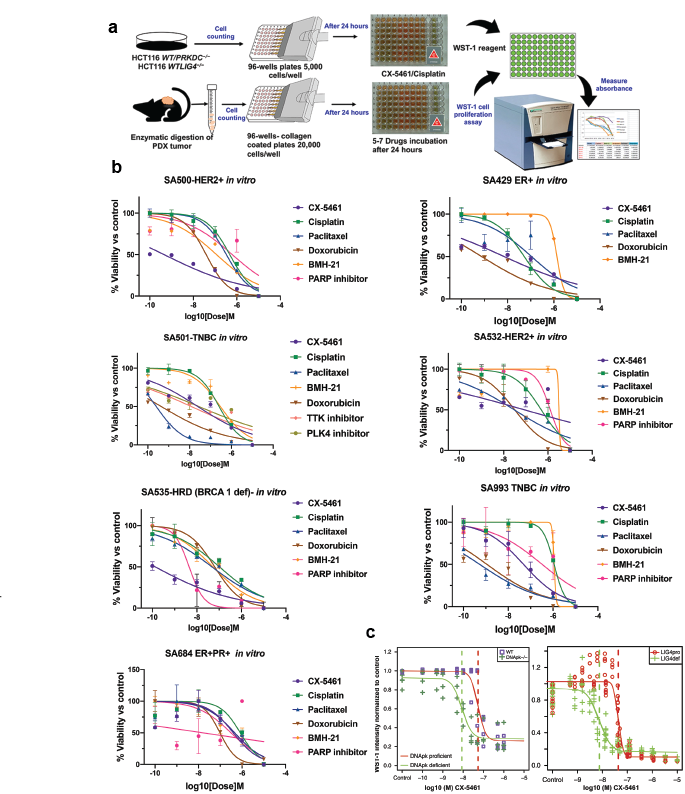
\includegraphics[width=\textwidth]{Figures/invitro.png}
	\caption[Drug efficacy testing \textit{in vitro} ]
	{\small
	    \textbf{Drug efficacy testing \textit{in vitro}.}
	    \textbf{(a)} Schematics of experimental design
	    \textbf{(b)} Examples of chemotherapies response \textit{in vitro} from PDX tumor cells. Horizontal axis a shows drug doses while vertical axis represents percent viability normalized to control
	    \textbf{(c)} Control HCT116 wt, DNApk KO and lig4 KO cell lines response to CX-5461. All horizontal axis represent drug doses while vertical axis shows percent viability normalized to control.
	}
	\label{fig:invitro}
\end{figure}
% Table generated by Excel2LaTeX from sheet 'in vitro screening'
\begin{table}[htbp]
  \centering
  \caption{Summary responses \textit{in vitro} screening}
    \begin{tabular}{llp{8.415em}}
    \hline
    \textbf{Drugs} & \textbf{PDX/ Cell lines } & \multicolumn{1}{l}{\textbf{Response}} \\
    \hline
    Paclitaxel & \multicolumn{1}{p{12.915em}}{SA429, SA500, SA501, SA532, SA535, SA684, SA993} & Dynamic dose dependent \\
    Docetaxel & \multicolumn{1}{p{12.915em}}{SA429, SA500, SA501, SA532, SA535, SA684, SA993} & Dynamic dose dependent \\
    Cisplatin & \multicolumn{1}{p{12.915em}}{SA429, SA500, SA501, SA532, SA535, SA684, SA993, HCT116 WT, HCT116 DNApk-/-, HCT116 lig4-/-} & Dynamic dose dependent \\
    Carboplatin & \multicolumn{1}{p{12.915em}}{SA500, SA532, SA535, SA684, SA993} & Dynamic dose dependent \\
    Doxorubicin & \multicolumn{1}{p{12.915em}}{SA429, SA500, SA501, SA532, SA535, SA684, SA993} & Dynamic dose dependent \\
    Fluorouracil (5-FU) & \multicolumn{1}{p{12.915em}}{SA500, SA501, SA532, SA535, SA684, SA993} & Less effective dose-dependent response \\
    Methotrexate & \multicolumn{1}{p{12.915em}}{SA500, SA501, SA532, SA535, SA684, SA993} & Less effective dose-dependent response \\
    Cyclophosphamide & SA500 & Less effective dose-dependent response \\
    Ifosfamide & SA500 & Less effective dose-dependent response \\
    CX-5461 & \multicolumn{1}{p{12.915em}}{SA429, SA500, SA501, SA532, SA535, SA684, SA993, HCT116 WT, HCT116 DNApk-/-, HCT116 lig4-/-} & Dynamic dose dependent \\
    CX-3543 & \multicolumn{1}{p{12.915em}}{SA429, SA500, SA501, SA532, SA535, SA684, SA993} & Dynamic dose dependent \\
    BMH-21 & \multicolumn{1}{p{12.915em}}{SA429, SA500, SA501, SA532, SA535, SA684, SA993, HCT116 WT, HCT116 DNApk-/-, HCT116 lig4-/-} & Dynamic dose dependent \\
    Pyridostatin & \multicolumn{1}{p{12.915em}}{SA429, SA501, SA532, SA535, SA684, SA993} & Less effective dose-dependent response \\
    Olaparib & \multicolumn{1}{p{12.915em}}{SA500, SA532, SA535, SA684, SA993} & Less effective dose-dependent response \\
    PLK4 inhibitor & SA501, SA532 & Less effective dose-dependent response \\
    TTK inhibitor & SA501, SA532 & Less effective dose-dependent response \\
    \hline
    \end{tabular}%
      \label{tab:addlabel}%
\end{table}%

\subsection{Short term \textit {in vitro} cultures reveals differential drug efficacy and PDX tissue responses
}
Next, we sought to establish drug efficacy of chemotherapies and G4 quadruplex, CX-5461, to determine the broad range of the PDX tumor responses in short term \textit{in vitro} assays. The purpose of these experiments is to judge the dynamics of responses from various PDX tumors in terms of therapeutic effectiveness before starting \textit{in vivo} screening. Total 7 PDX tumors, including 3 TNBC, 2 ER+ and 2 HER2+, were enzymatically digested into single cells and plated in 96-well collagen coated plates  \textbf{\autoref{fig:invitro} a, See methods}. 
Our results in tumor cultures showed dynamic range of responses across multiple PDX towards various chemotherapies while few of them tend to be less effective \textbf{(Summary results in table 3.1, representative response curves in \autoref{fig:invitro} a}. Doxorubicin in contrast showed very toxic behavior. A new compound of our interest, CX-5461 also revealed a high efficacy with wide range of responses across different PDX tissues \textbf{\autoref{fig:invitro} b}. Another compelling finding from CX-5461 was from the control cell lines, HCT116, that showed differential responses to CX-5461 with deficient DNA repair pathways \textbf{\autoref{fig:invitro} c}. These mechanisms were later explored in detail in the lab and was published by Xu \textit{et al}, \cite{xu2017cx}. 


% Table generated by Excel2LaTeX from sheet 'table for R'
\begin{table}[htbp]
  \centering
  \caption{PDX tumors \textit{in vivo} screening with 3x1x1}
    \begin{tabular}{lllll}
    
     \hline
    \textbf{Tumor ID} & \textbf{Cisplatin} & \textbf{Paclitaxel} & \textbf{Rucaparib} & \textbf{CX-5461} \\
     \hline
    SA532 & N/A   & N/A   & N/A   & Sensitive \\
    SA535 & Sensitive & Sensitive & Partially-Sensitive & Sensitive \\
    SA605 & Sensitive & Sensitive & N/A   & N/A \\
    SA604 & Sensitive & Sensitive & Resistent & Resistent \\
    SA609 & Sensitive & Sensitive & Resistent & Resistent \\
    SA919 & N/A   & Sensitive & N/A   & N/A \\
    SA920 & N/A   & N/A   & N/A   & Resistent \\
    SA993 & N/A   & N/A   & N/A   & Sensitive \\
    SA995 & N/A   & N/A   & N/A   & Partially-Sensitive \\
    SA1035 & Sensitive & Partially-Sensitive & Resistent & Sensitive \\
    SA1130 & Sensitive & N/A   & N/A   & Sensitive \\
    X2371 & Sensitive & Partially-Sensitive & N/A   & Sensitive \\
    X2440 & Sensitive & Sensitive & N/A   & N/A \\
     \hline
    \end{tabular}%
    
PDX ID = Patient-derived xenograft identification, N/A = Not applicable\\
  \label{tab:addlabel}%
\end{table}%
\begin{figure}
	\centering
	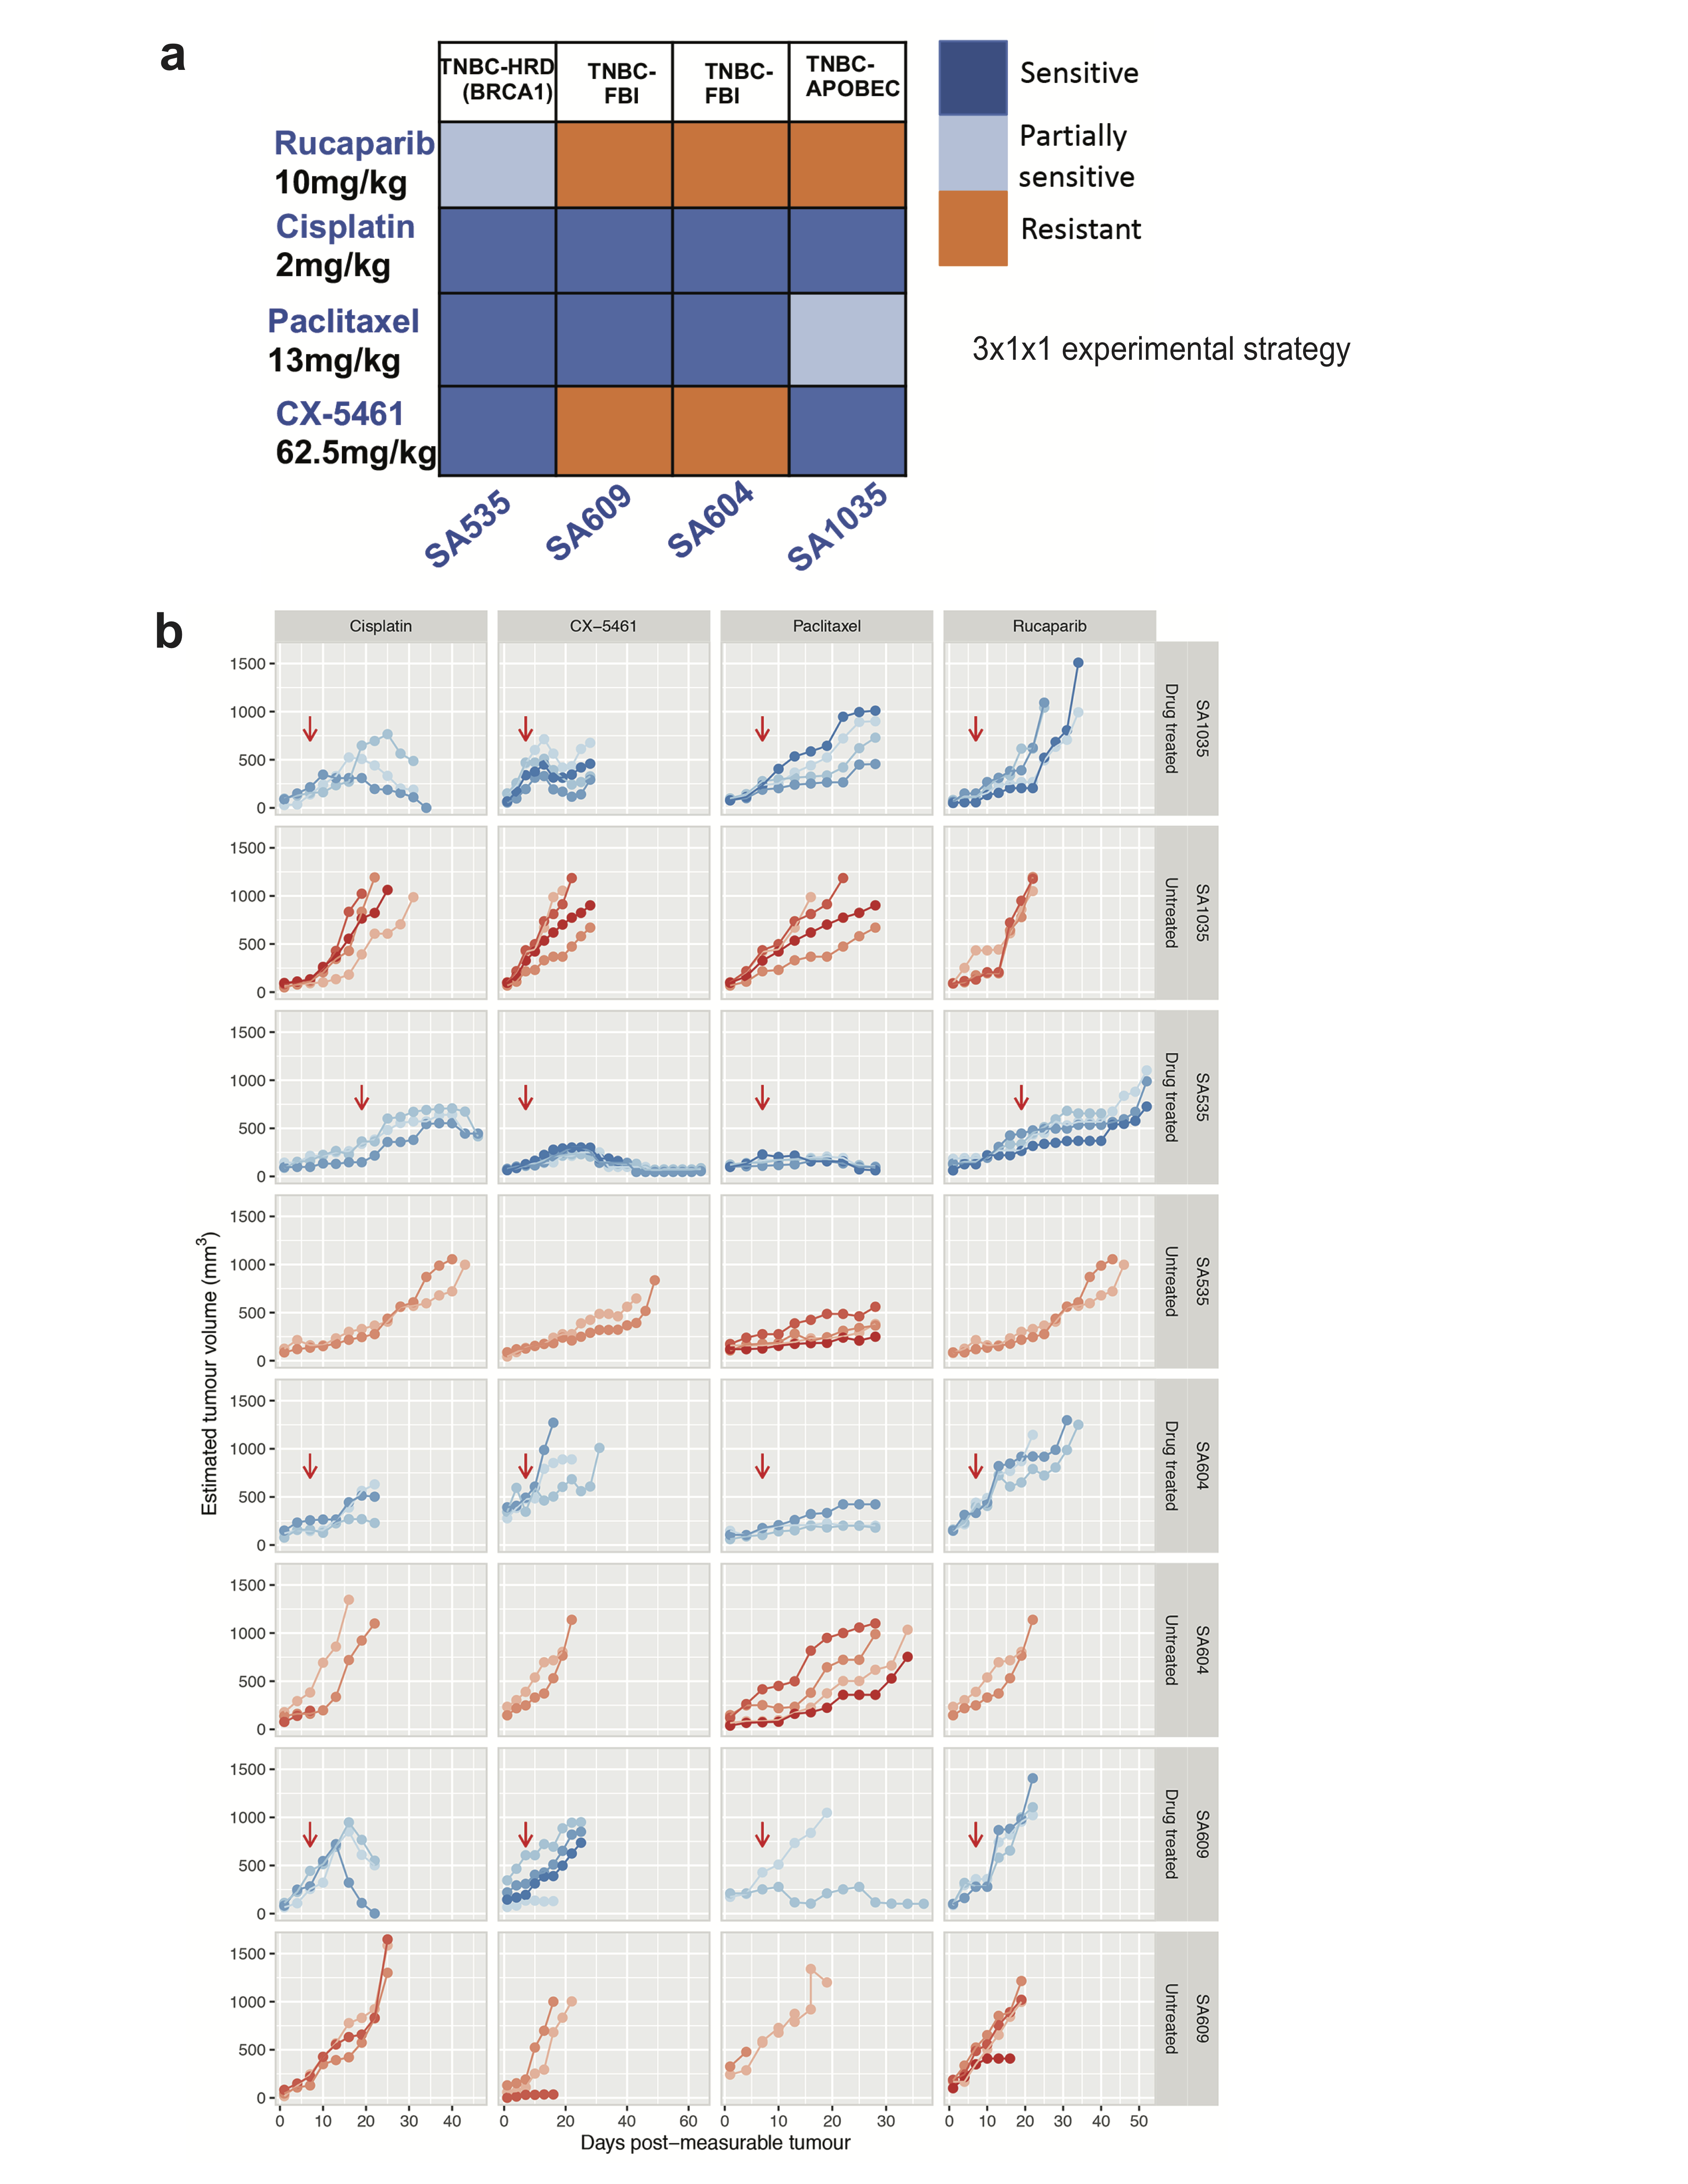
\includegraphics[width=\textwidth]{Figures/4drugs4PDXNew.png}
	\caption[Representative tumor responses from four PDX and  to four drugs]
	{\small
	    \textbf{Representative tumor responses from four PDX and  to four drugs.}
	    \textbf{(a)} Summary matrix of four TNBC PDX with drugs
	    \textbf{(b)} Tumor growth curves from treated and un treated tumors. Vertical axis representing the tumor volume in cubic millimeters and horizontal axis is showing the days tumor measurements. Red arrows represent the time of start of treatments.
}
	\label{fig:EstablishmentofPDX}
\end{figure}


\begin{figure}
	\centering
	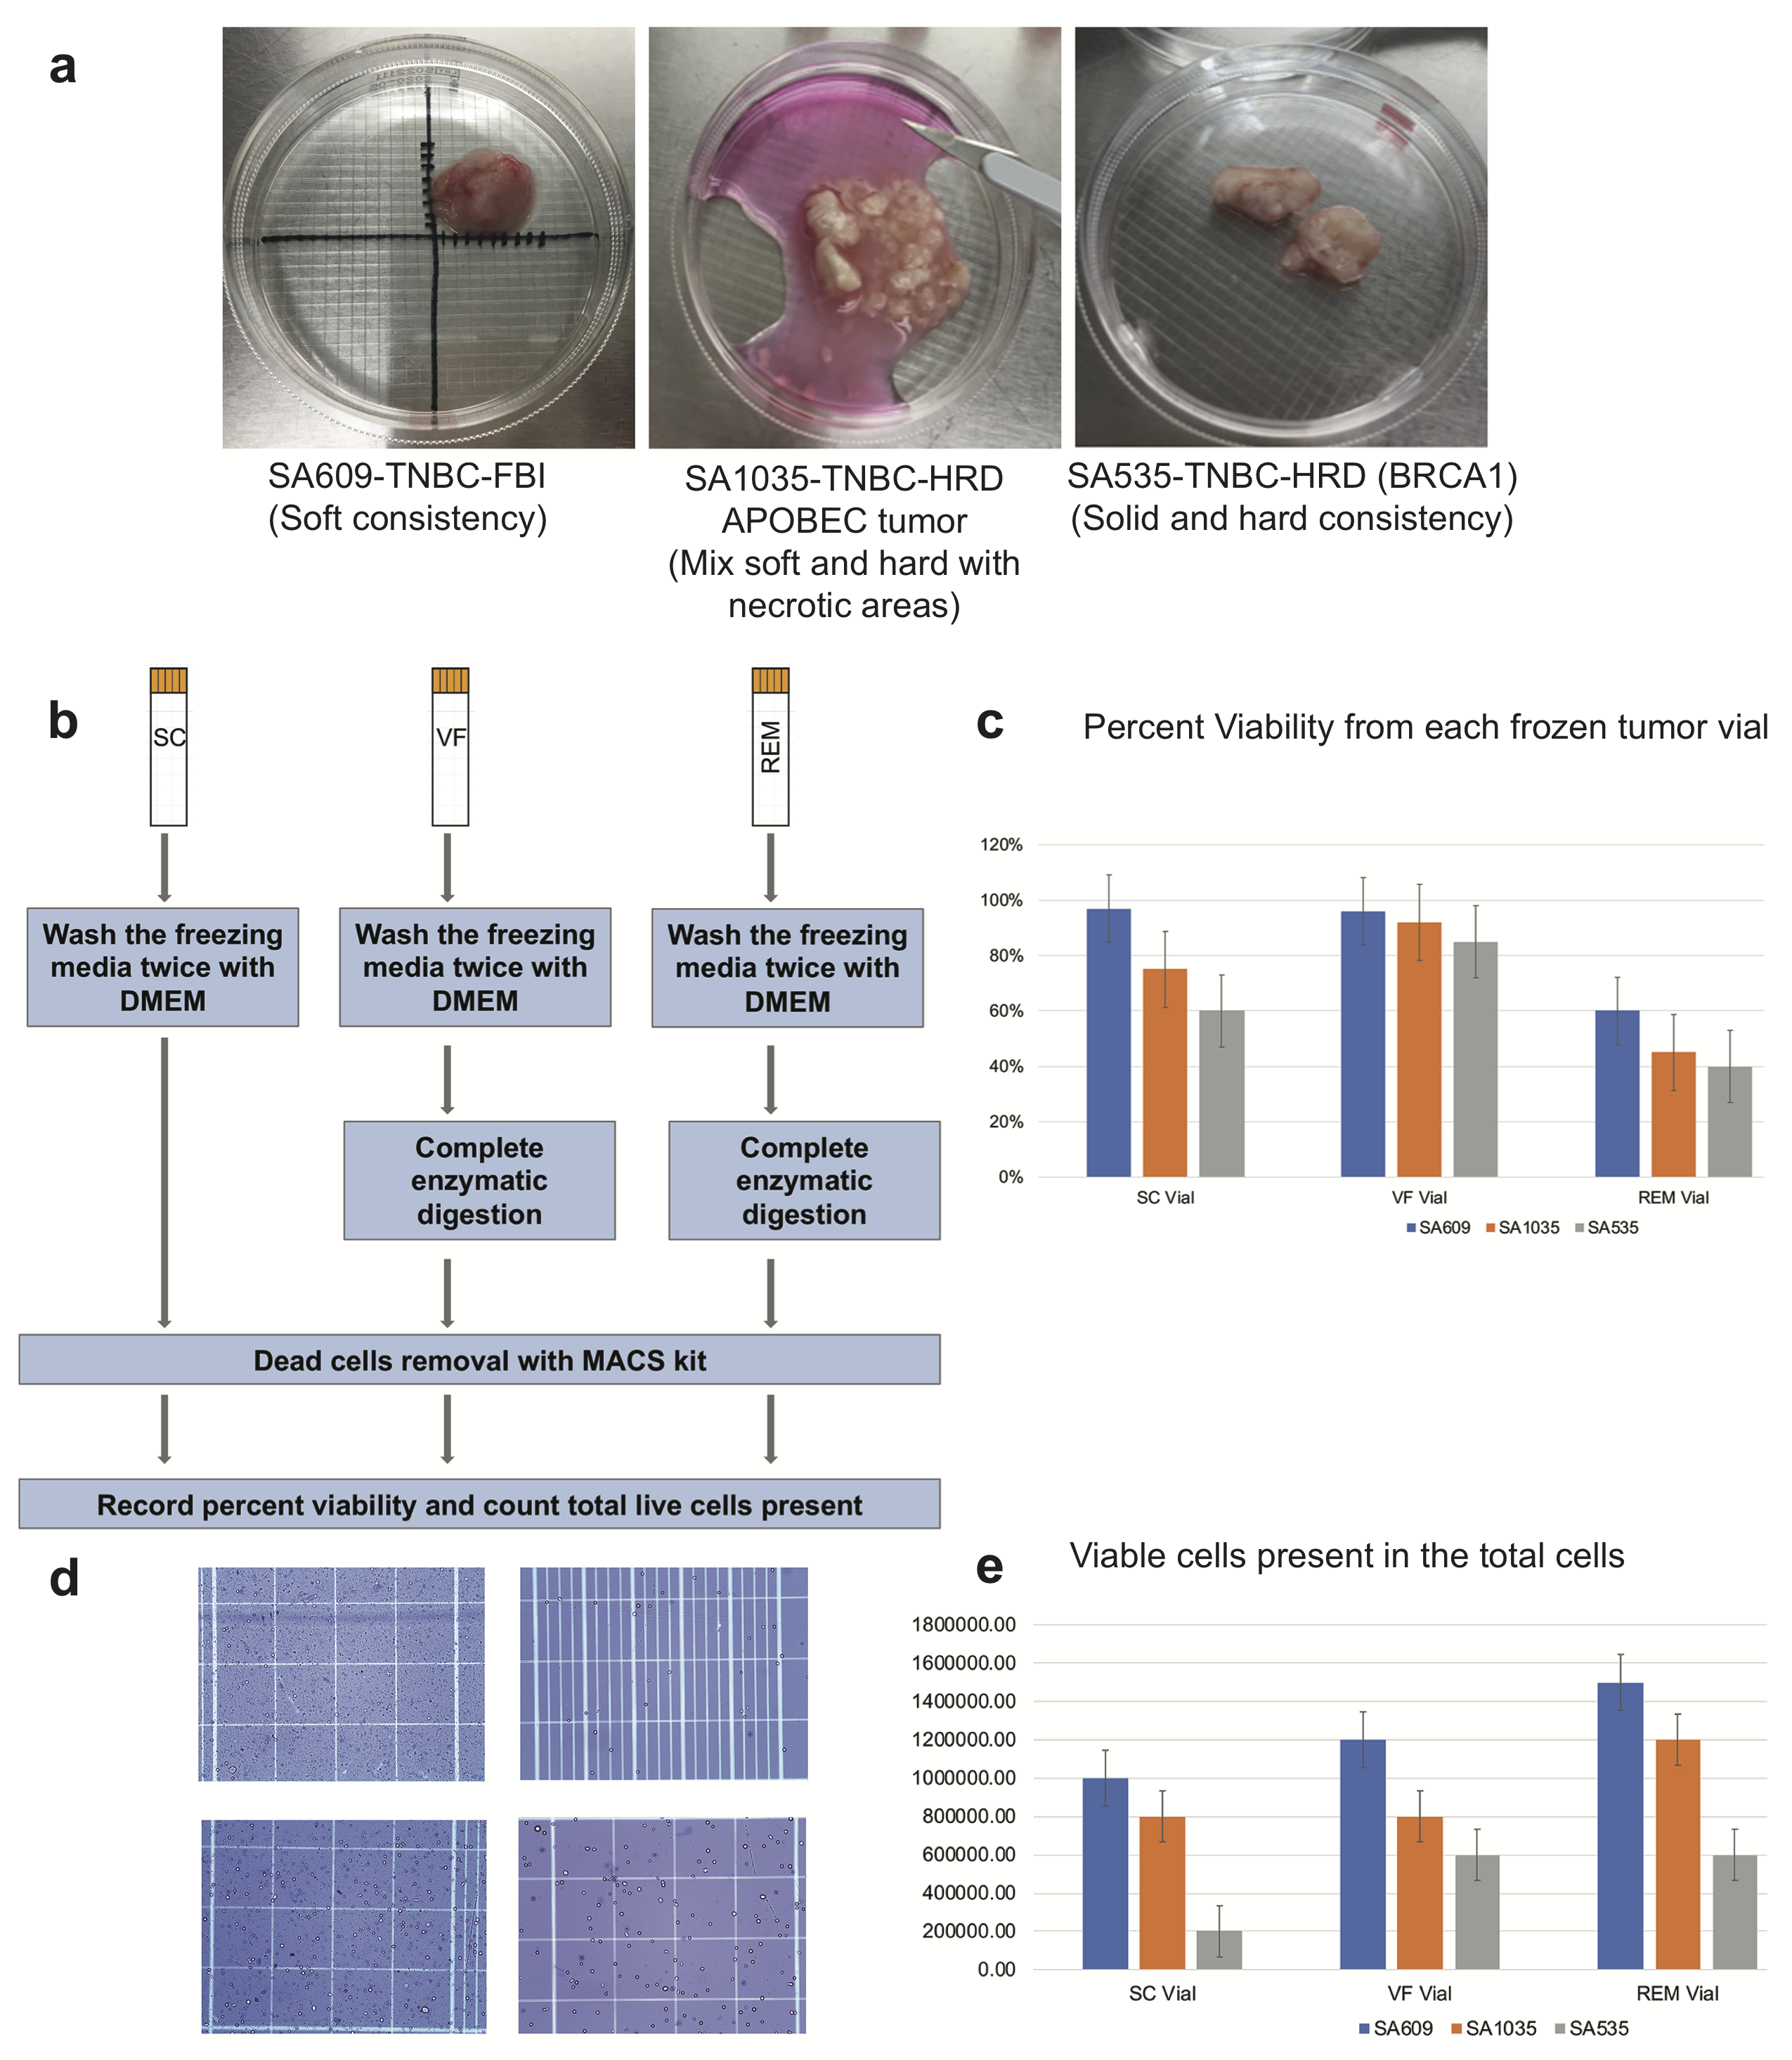
\includegraphics[width=\textwidth]{Figures/cellviability2.png}
	\caption[Evaluation of viable-high percent cell recovery for single cell measurements]
	{\small
	    \textbf{Evaluation of viable-high percent cell recovery for single cell measurements.}
	    \textbf{(a)} Representative tumors in dishes. Left side dish has black lines showing area between two small lines as 2mm. Middle dish showing partially chopped tumor with white necrotic tissues. Right side panel showing example from comparatively solid to cut tumor.
	    \textbf{(b)} Schematics of processing the frozen vials \textbf{(also see methods)}
	    \textbf{(c)} Vertical axis showing the percent viability and horizontal axis shows the type of vials from each of three tumors  \textbf{(d)} Left sided images are pre dead cell removal while right sided are the post dead removal \textbf{(e)} Vertical axis showing the number of viable cells obtained from each vial and horizontal axis shows type of vials processed.
	}
	\label{fig:cellviability}
\end{figure}


\subsection{Baseline \textit{in vivo} sensitivity patterns of triple negative breast cancer }
In order to determine the baseline sensitivity of PDX tumors with conventional and novel targeted chemotherapies. We modified the approach laid out in literature for PDX sensitivity testing and performed \textit{in vivo} screen on to model inter-patient response heterogeneity with \textbf{three animals per model per treatment strategy (3x1x1)} \cite{gao2015high,migliardi2012inhibition}. For this purpose, 13 PDX were tested with chemotherapies \textbf{(Summary in table 3.2)} and the response patterns were recorded. 
\textbf{Figure 3.3 a} showing summary matrix of four triple negative breast (TNBC) PDX towards chemotherapies. We selected in total four drugs, two standard chemotherapies, including platinum (cisplatin-(2mg/kg, Q3Dx8 i.p. max)) and Taxanes (Paclitaxel-13mg/kg, Q3Dx8 i.p. max), and two targeted chemotherapies, including PARP inhibitors (Rucaparib-IP daily 5 days per week for 3 weeks) and G4 quadruplex stabilizers (CX-5461-62.5mg/kg, Q3Dx8 by oral gavage max).  The representative grrowth curves are shown in \textbf{figure 3.3 b}, including SA609 (Basal, TP53, FBI), SA1035 (Basal, HRD, APOBEC-like, POLH), SA535 (Basal, MMRD-1, S-Dup, TP53, BRCA1 def) and SA604 (Basal, CI-SV, CI-FBI).
Interestingly, we found that all TNBC PDX with different background mutational signatures behaved differently towards the same drugs. SA609 and SA604 were both found to be resistant to the new compound CX-5461 as well as Rucaparib.
All four of the PDX showed high sensitivity to platinum (cisplatin) while three out of four were sensitive to (taxane) paclitaxel. 


\subsection{Optimization methods in isolation, disaggregation and freezing of PDX tissues for single cell analysis}

Next we investigated how can we get maximum number of good quality cells for single cell sequencing. Subsequently, we compared the effect of tumor dissociation with collagenase at high temperature versus dissociation at low temperature with cold active protease on transcriptomes.

\subsubsection{Small viable frozen fragments of the tumors culminated in high viability and less debris as compared to big frozen chunks}
To investigate which status of tissue freezing will give us better outcome of single cell suspension, we mechanically disaggregated three TNBC PDX tumors \textbf{(Figure 3.4 a)}, SA609, SA1035 and SA535 and froze them by three different ways. First, after mechanical digestion, viable frozen (VF) tissue fragments were frozen in the freezing media. Second frozen vial consist of single cells (SC) by complete enzymatic digestion \textbf{(See methods)} and lastly big tissue chunks frozen vial labelled as "REM" (remaining). Tumor fragments in the vials labelled with "VF", "REM" and already digested fragments stored as "SC", were thawed and washed twice with the media. VF and REM fragments were digested to single cells with collagenase hyaluronidase and dead cells and debris were removed from all the single cells final suspension as described in the method section \textbf{(Figure 3.4 b)}. We obtained high percent viabilty from viable frozen tumor fragments across all the three tested PDX tumors scoring approximately from 82\% to 95\% as compared to the others \textbf{(Figure 3.4 c)}. However, the final number of viable cells in each of the specific vial across different PDX varies from 200 thousands to one million 400 thousands  \textbf{(Figure 3.4 e)}.  Interestingly, one of the PDX tumor, TNBC-SA609 turns out to be behaving comparatively effectively under every condition. 
Finally, in order to  remain consistent across every type of tumor, we concluded that Viable frozen "VF" tissue vial is the best option giving us moderate number of viable cells across xenografts. Also, we found that dead cell removal step gives us an additional layer of purity as it was accompanied by debris clean up \textbf{(Figure 3.4 d)}.



\subsubsection{Dissociation with Collagenase at 37\textdegree C induces a distinct stress response in single-cell transcriptomes}
To uncover transcriptional variation and responses to dissociation method and to see the effect of digestion temperature on the transcriptome, we generated scRNA-seq data from a range of PDX tumors dissociated at low temperature with cold active protease and at high temperature with collagenase and Hyaluronidase, using the 10x Genomics Chromium v3 platform \textbf{(see methods)}.
We performed a differential expression analysis on the 23,731 cells found by combining all experiments measured in PDX tumors at either 6$^{\circ}$°C or 37$^{\circ}$°C. After retaining genes with at least 10 counts across all cells, we performed differential expression analysis with edgeR \cite{robinson2010edger}, while controlling for the sample-of-origin.
We found that of the 19,464 genes retained for analysis, 11,975 (62\%) were differentially expressed at a Benjamini-Hochberg corrected false discovery rate (FDR) of 5\%. We defined a core set of genes meaningfully perturbed by digestion temperature as those significantly differentially expressed as above, but with an absolute log fold change of at least 1.5. Therefore, for a gene to be included under these criteria it must be differentially expressed and its abundance increased or decreased by at least 50\% by digestion temperature. 



\begin{figure}
	\centering
	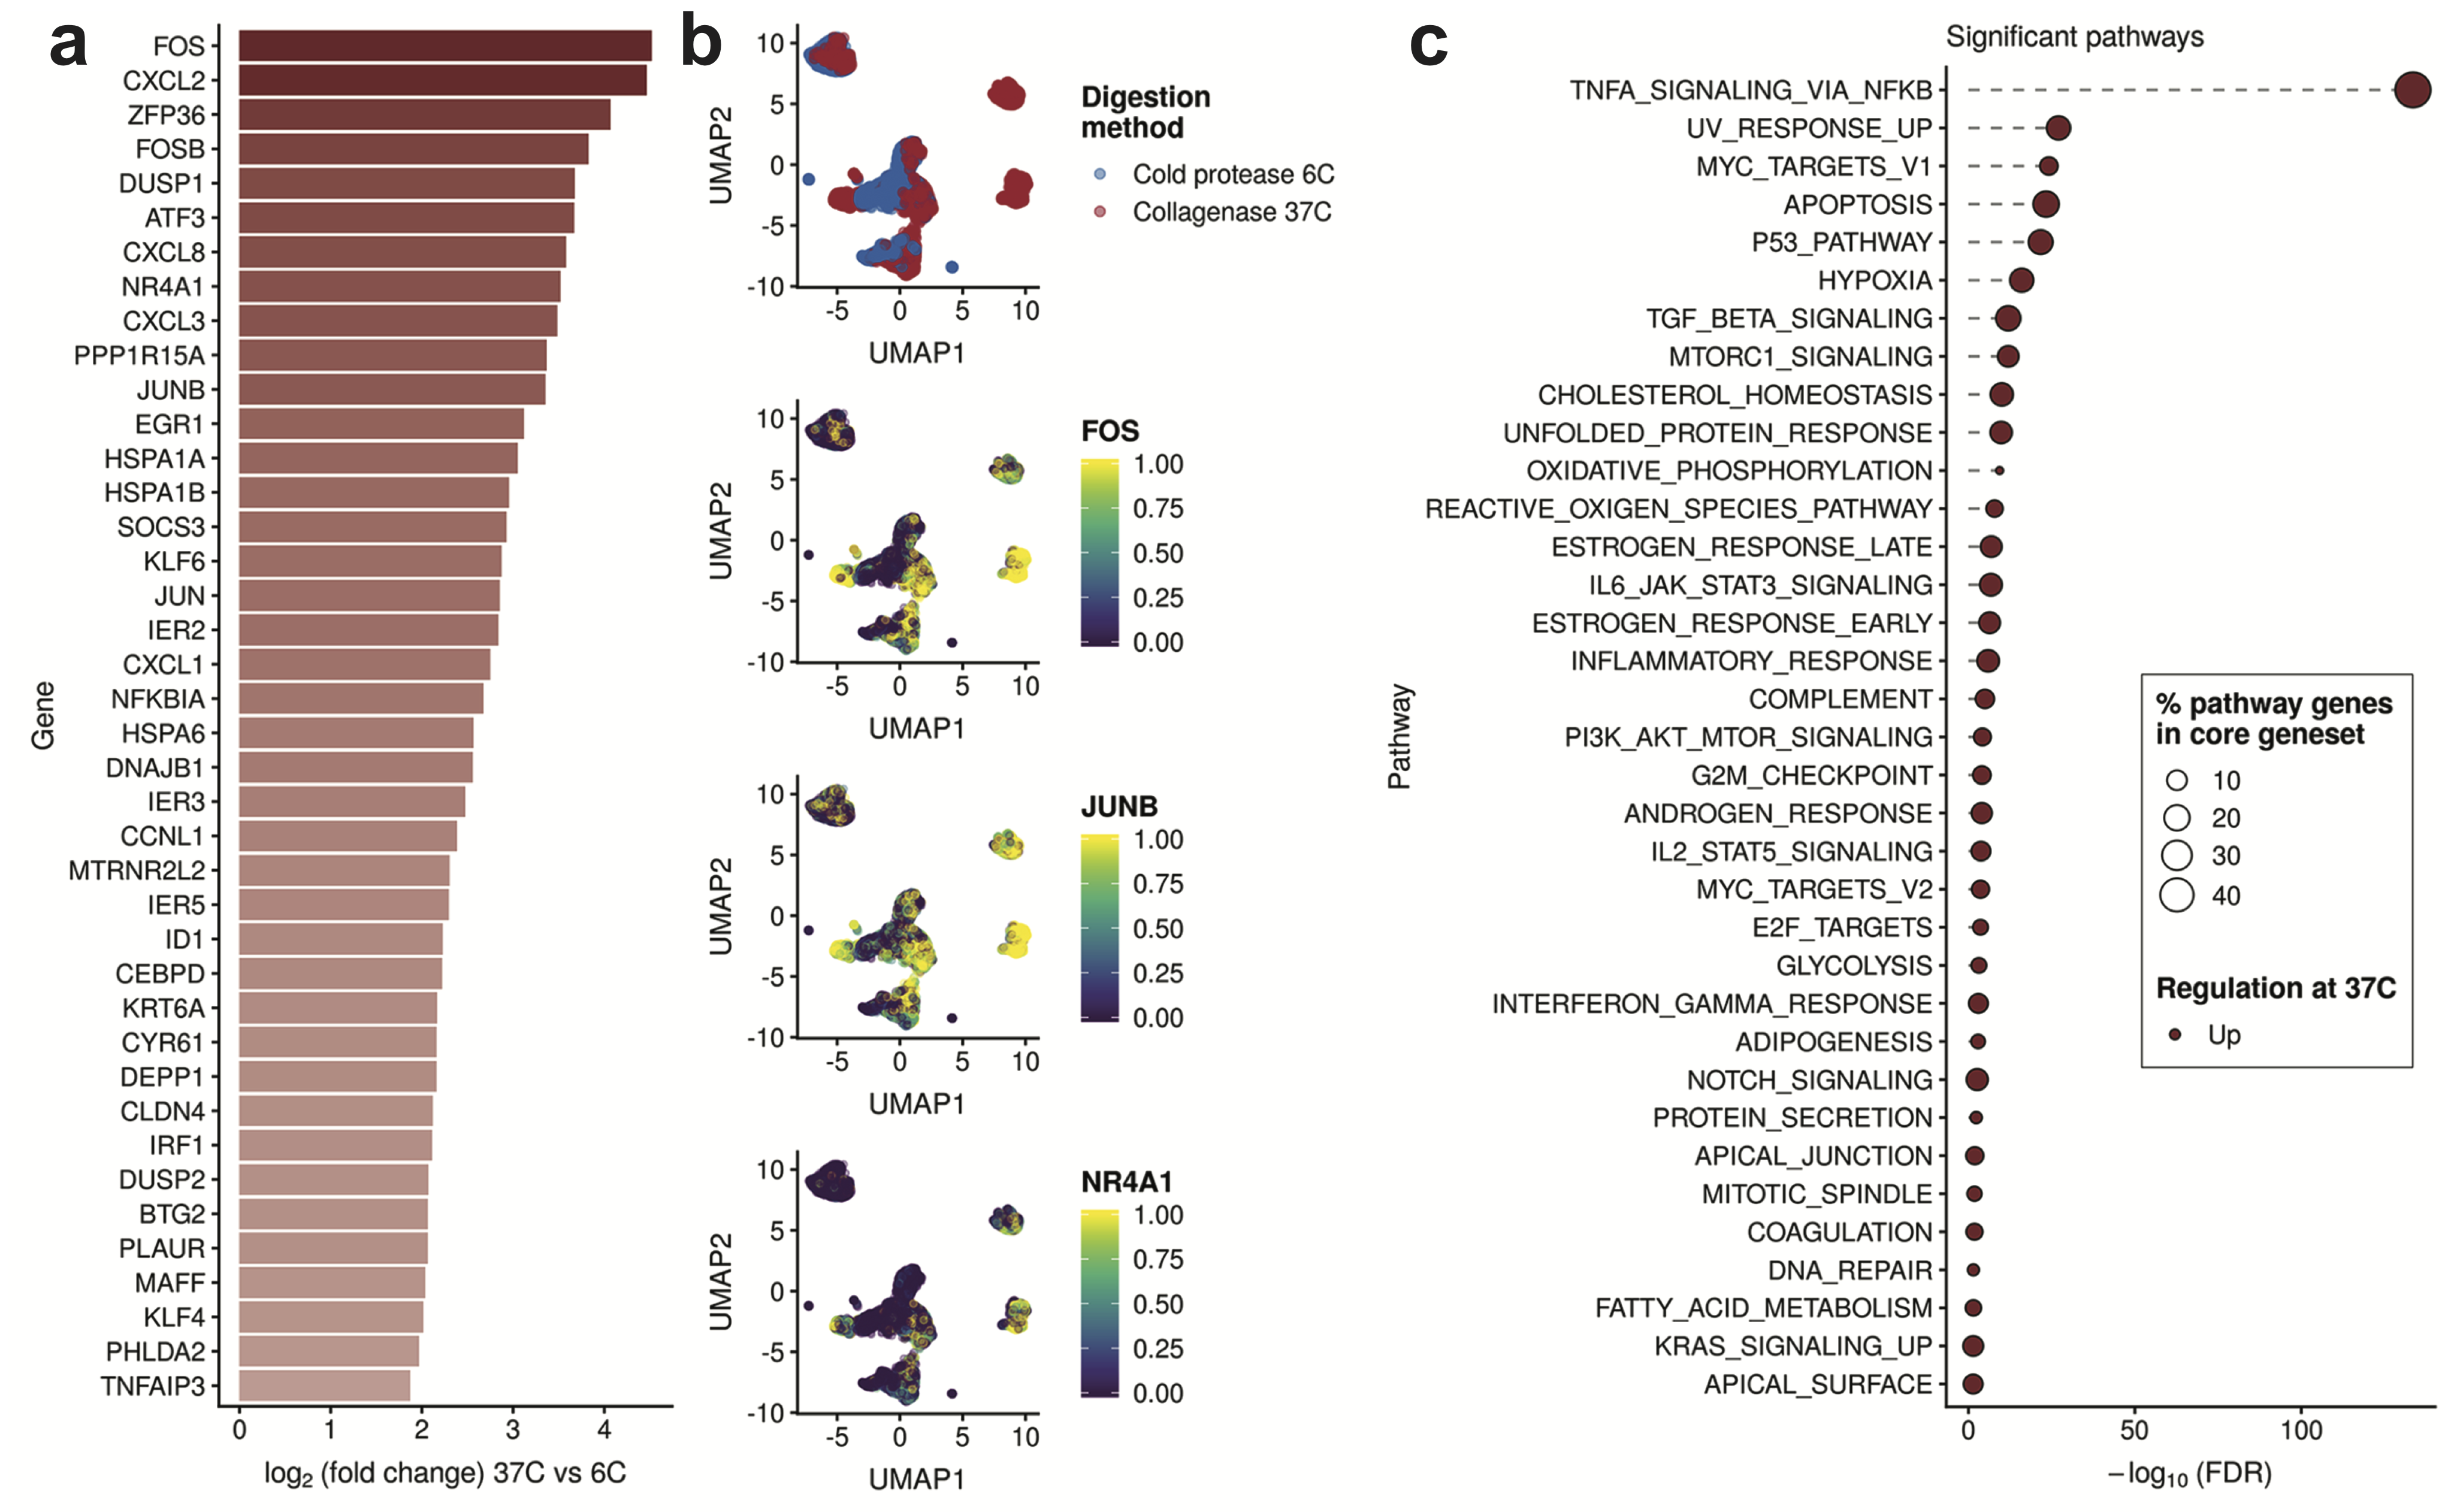
\includegraphics[width=\textwidth]{Figures/stressresponse1.png}
	\caption[Dissociation with collagenase induces a distinct stress response in PDX tumors]
	{\small
	    \textbf{Dissociation with collagenase induces a distinct stress response in PDX tumors.}
	    \textbf{(a)} The top 40 genes (by log fold-change) from the 11,975 identified as significantly differentially expressed between cells digested at 6\textdegree C and 37\textdegree C.
	    \textbf{(b)} UMAP plots of 23,731 cells coloured by digestion temperature (top) then by normalized expression of 3 key stress response genes (\emph{FOS}, \emph{JUNB}, \emph{NR4A1}) demonstrates a distinct concordance between temperature and induction of the stress gene signature.
    Expression values are log normalized counts winsorized to $[0,2)$ then scaled to $[0,1)$
	    \textbf{(c)} Pathway analysis of differentially expressed genes with the MSigDB hallmark gene sets highlights induction of genes involved in NF-$\kappa$B signalling at 37\textdegree C digestion with 46.5\% of 200 genes annotated in the pathway being found in the 512 core gene set}
	\label{fig:stressresponseinpdx}
\end{figure}

This produced a core gene set of 512 genes, of which 507 were upregulated at 37$^{\circ}$ C and the remaining 5 downregulated. This gene set includes multiple canonical stress-related genes such as \emph{FOS}, \emph{FOSB}, \emph{ATF3} and heat shock proteins (HSPs) \textbf{(Figure 3.5 a)}, expression of which have shown to be induced by collagenase dissociation in a subset of muscle cells \cite{van2017single}. A UMAP embedding of the cells coloured by dissociation temperature and the expression of several key genes (\emph{FOS}, \emph{JUNB}, \emph{NR4A1} \textbf{(Figure 3.5 b)}, further demonstrates the digestion temperature-specific induction of the expression of these genes.
We subsequently performed a pathway enrichment analysis on the differential expression results, searching for enrichment in given hallmark pathways \cite{liberzon2015molecular} \textbf{(Figure 3.5 c)}. Of particular note was TNF (tumor necrosis factor) signalling via NF-$\kappa$B of which 46.5\% of annotated pathway genes were included in the core set of 512 genes.Further enrichment of stress-associated pathways including hypoxia, apoptosis, and inflammatory response is further indicative of collagenase dissociation at 37$^{\circ}$°C as inducing a stress response on the transcriptomes of single cells.


 \subsubsection{Identification of subpopulations of dead, dying and live cells in transcriptomic data}
Given the bi- and tri-modal distributions of mitochondrial gene count percentages apparent in the PDX experiments and previous studies' assertions that high mitochondrial gene content is indicative of dead and dying cells \cite{ilicic2016classification, zhao2002mitochondrial}, we next sought to determine the contribution of dead and dying cells to the variation observed in QC metrics in \cite{o2019dissociation}. In order to induce classical cell death pathways, we used TNF\textalpha \cite{carswell1975endotoxin, sedger2014tnf} to treat the non tumourigenic, lymphoblastoid cell line GM18507 and FACS sorted cells into dead or and dying fractions based on PI/Annexin V positivity \textbf{(Figure 3.6 a)}, as well as a live, untreated fraction. Notably, cell yield from scRNAseq data was highly dependent on the cell status, with 8,597 live cells recovered but only 1,280 and 885 dead and dying respectively compared to targeted numbers of 3,000 cells. 
A principal components analysis (PCA) following mutual nearest neighbours (MNN) correction \cite{haghverdi2018batch} demonstrated the cells approximately segregating along the first principal component (PC1) by cell status \textbf{(Figure 3.6 b)}, albeit with high levels of heterogeneity in overlap. Indeed, PC1 closely tracked the mitochondrial gene content of the cells \textbf{(Figure 3.6 c)}, being significantly higher in dead cells (median 29.9\%) compared to both dying cells (median 3.13\%, $p=$ 1.17e−126) and live cells (median 3.4\%, $p=$4.65e−153) as shown in \textbf{Figure 3.6 d}.
This observation justifies the practice of excluding cells with very high mitochondrial gene content as being likely dead cells.

\begin{figure}
	\centering
	\includegraphics[width=\textwidth]{Figures/livedead.png}
	\caption[Transcriptomic landscape of live, dead, and dying cells.]
	{\small
	    \textbf{Transcriptomic landscape of live, dead, and dying cells.}
	    \textbf{(a)} FACS analysis showing gating strategy for untreated, live cells (PI−/annexin V−) or TNFα-treated dying cells (PI/annexin V+) and dead cells (PI+/annexin V+).
	    \textbf{(b)} PCA projection of the three cell conditions showing approximate segregation of cell status along the first principal component (PC1), with live and dying cells enriched at lower PC1 values and dead cells enriched at higher values.
	    \textbf{(c)} PCA projection colored by the percentage mitochondrial genes (“\% transcriptome mitochondrial”) shows significant increase along the PC1 \textbf{(d)} Dead cells exhibit significantly higher percentage of the transcriptome as mitochondrial compared to both live and dying cells \textbf{(e)} Unsupervised clustering of the gene expression profiles clusters the cells into three groups, approximately tracking both PC1 of the data and the percentage of transcriptome mitochondrial\textbf{(f)}The composition of each cluster demonstrates that cluster 1 is primarily composed of live cells, cluster 2 a mix of live, dying, and dead cells, while cluster 3 is composed mainly of dead cells \textbf{(g)} The \% transcripts mitochondrial is significantly different between the three clusters, with a step increase in proportion moving from cluster 1 to 2 and 2 to 3 \textbf{(h)} Cluster 2 significantly up-regulates the MHC class I gene set, suggesting it represents stressed or pre-apoptotic cells.
	}
	\label{fig:cellviability}
\end{figure}



\begin{figure}
	\centering
	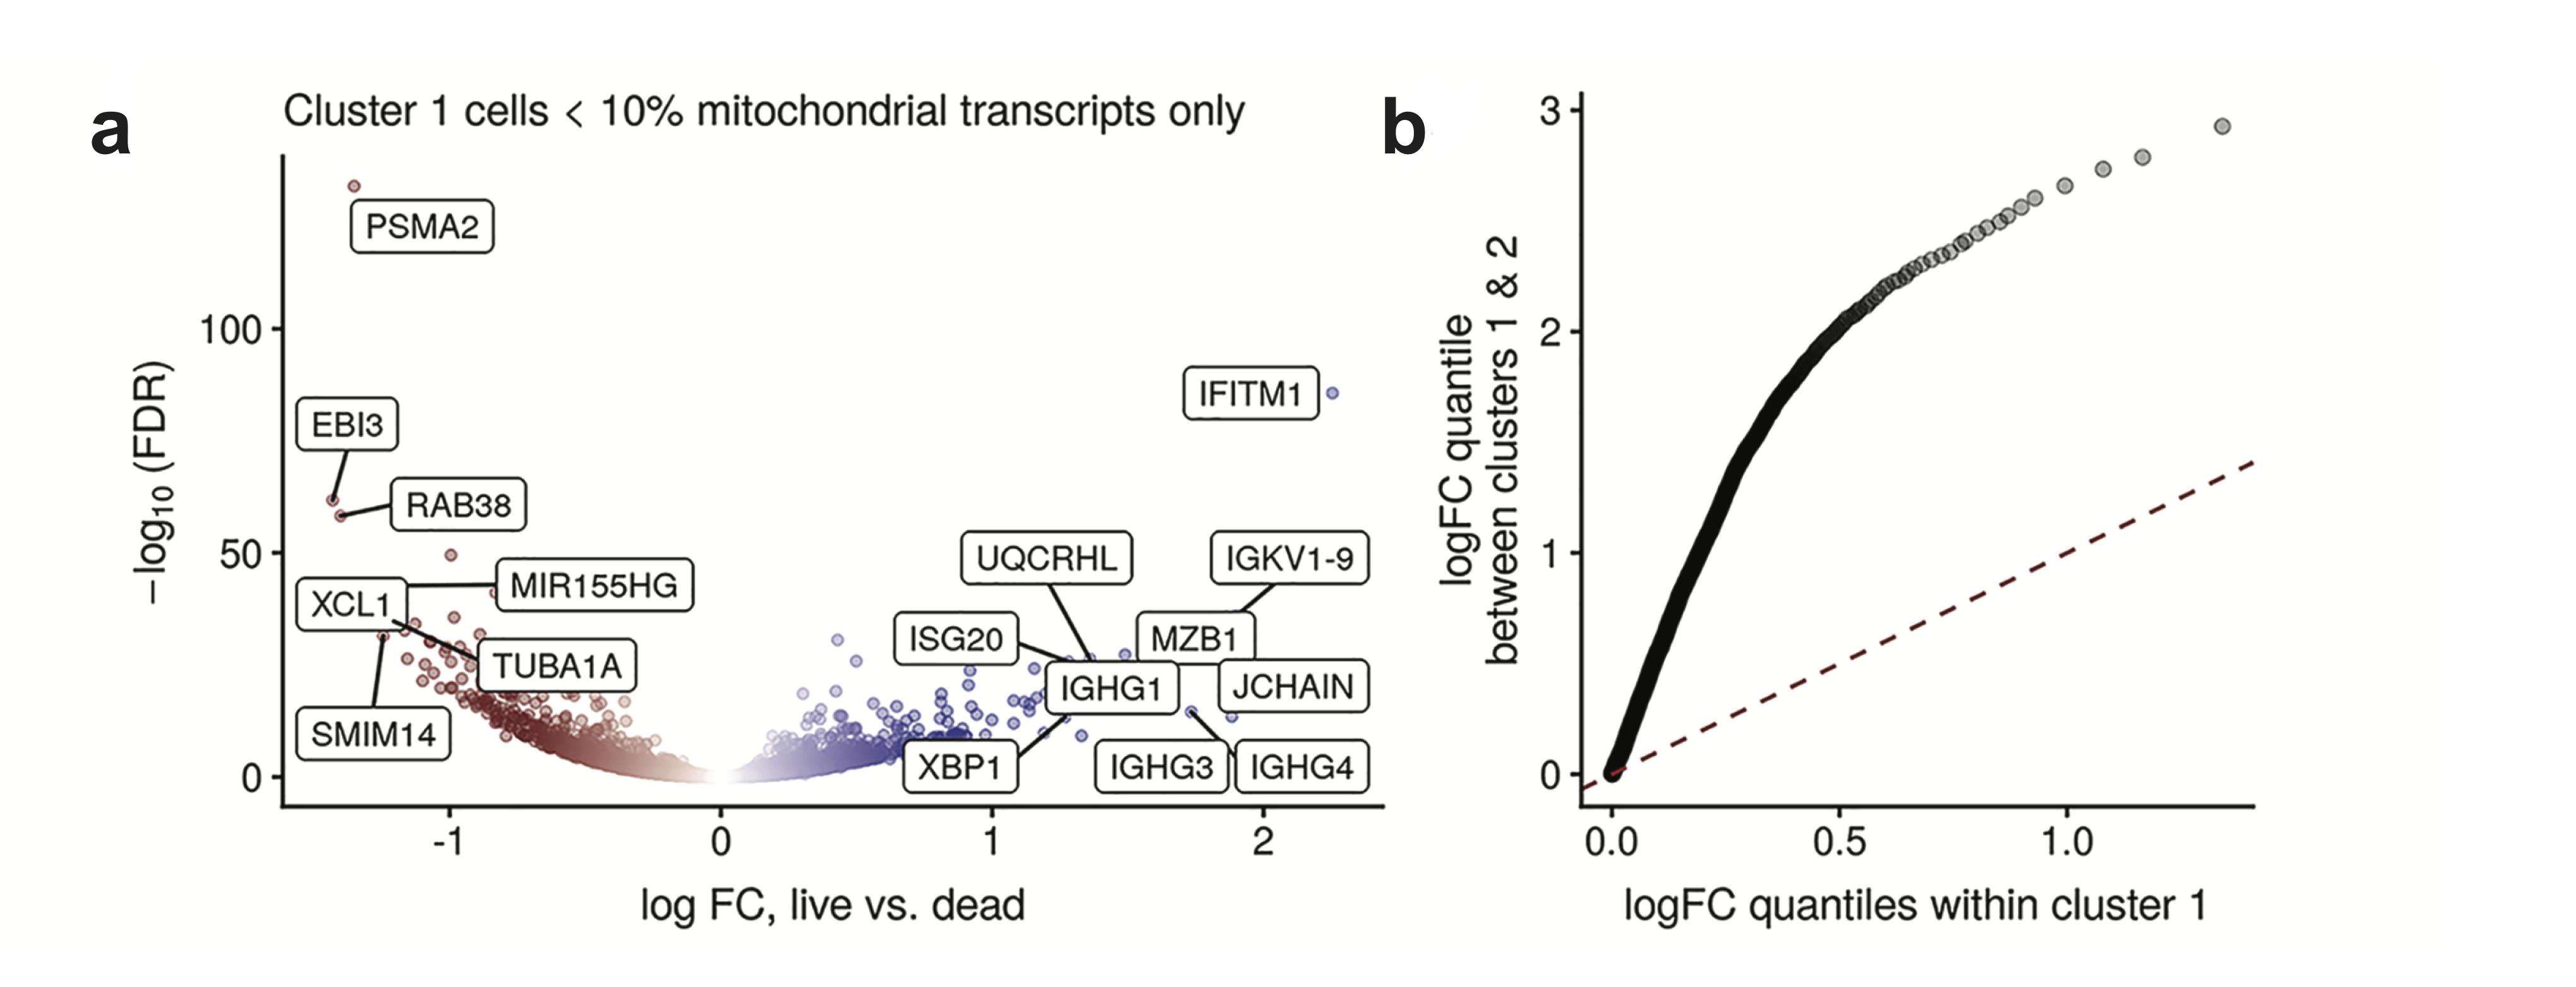
\includegraphics[width=\textwidth]{Figures/livedead2.png}
	\caption[Differential expression of cluster 1 of live, dead, and dying cells.]
	{\small
	 \textbf{Differential expression of cluster 1 of live, dead, and dying cells.}
    \textbf{a} Differential expression analysis of transcriptomically ``healthy'' cells within cluster 1 reveals residual differences between cells sorted as live and dead.
    \textbf{b} The distribution of absolute effect sizes (log fold change) of live vs. dead cells within cluster 1 (x-axis) compared to between clusters 1 and 2 (y-axis) demonstrates the residual effect on the transcriptome of being live/dead sorted is small compared to the inter-cluster expression variance.	}
	\label{fig:cellviability}

\end{figure}


Having observed that the transcriptomes of the different cell conditions are not entirely distinct, we sought to discover the extent of mixing between transcriptomic states and whether live and dead cells that appear transcriptomically ``healthy'' (i.e would ordinarily pass QC) are distinguishable. Using hierarchical clustering (methods) we clustered the cells into 3 groups  that approximately track PC1  \textbf{(Figure 3.6 e)}. Interestingly, these three groups show variable composition in terms of cell states, with cluster 1 being comprised mainly of live cells 86\% live, 8.5\% dying, 5.1\% dead), cluster 2 containing an increased proportion of dying and dead cells (68\% live, 7.5\% dying, 24\% dead), and cluster 3 comprised mainly of dead cells 5.9\% live, 6.7\% dying, 87\% dead).  Furthermore, we observed a step change increase in mitochondrial gene content between clusters \textbf{(Figure 3.6 g)}, with cluster 1 having the lowest (median 3.13\%), followed by cluster 2 having a significant increase (median  26\%, $p=$ 0) and cluster 3 having a significant increase beyond that (median 82.2\%, $p=$ 2.35e−149). Differential expression analysis between these clusters revealed a significant up-regulation in stress-associated pathways such as MHC class I  \textbf{(Figure 3.6 h)} in cluster 2 compared to clusters 1 \& 3. MHC class I genes are involved in antigen presentation to T cells, but are also expressed in many cell types and are induced in response to stress stimuli and contain heat shock-inducible elements \cite{gleimer2003stress}. 

Together, these results suggest a model whereby cluster 1 represents transcriptomically ``healthy'' cells, cluster 2 represents transcriptomically stressed cells that upregulate stress pathways  and have increased mitochondrial gene content (due to either an increasingly permeable membrane causing loss of cytoplasmic mRNA or increased metabolic demands), and cluster 3 represents transcriptomically dead cells whereby the membrane has burst leaving majority mitochondrial transcripts. Importantly, cells that are FACS sorted as either live, dying, or dead, are present in all three clusters, highlighting that the transcriptomic state of the cell is not necessarily the same as the surface marker state (though the two are correlated). Such concepts are reminiscent of ``pseudotime'' in single-cell developmental biology, whereby developmentally ordering cells transcriptomically can lead to early or late cells being placed at variable positions along the pseudotime trajectory \cite{campbell2018descriptive,campbell2018uncovering}. Indeed, PC1 from \textbf{Figure 3.6 a} approximates a pseudotime trajectory through the data, that tracks transcriptomically healthy cells to transcriptomically dead cells with increasing PC1 values.

Finally, we sought to determine if a sorted dead cell that appears transcriptomically healthy remains distinguishable from a sorted live cell in the transcriptomically healthy group. Using only cells in cluster 1, we further subsetted them to pass a strict set of QC filters (at least $10^3$ total genes detectable, \% mitochondrial content between 1 and 10) and performed a differential expression analysis between cells sorted as live and dead in this group. Of the 10,537 genes retained for analysis, 2,130(20.2\%) were found to be differentially expressed \textbf{(Figure 3.7 a)}, including downregulation of \emph{IFITM1} in dead cells. To compare this type of variation to the inter-cluster transcriptomic variation, we performed a second differential expression analysis between clusters 1 and 2, finding 8835 of 10,933 (80.8\%) genes significantly differentially expressed. Furthermore, the effect sizes were significantly larger for the inter-cluster comparison than the within-cluster 1 live-dead comparison as demonstrated by the quantile-quantile plot of absolute effect sizes in the \textbf{Figure 3.7 b}. Together, these results suggest that though there are gene expression differences between dead and live sorted cells within cluster 1, the magnitude of expression variation is small compared to transcriptomically stressed clusters.
 
 \subsubsection{Transcriptomic stress response is induced by both digestion time and digestion temperature}
To determine whether the gene signature identified above was induced due to the longer digestion time required for complete collagenase dissociation or due to the enzyme itself, we conducted a time course experiment, incubating breast PDX tissue with collagenase or cold protease for up to 3 hours. Since proteases work at different speeds on intact tissues, single cells released into the supernatant were sampled at 30 minutes, 1 hour, 2 hours or 3 hours.   
 

\begin{figure}
	\centering
	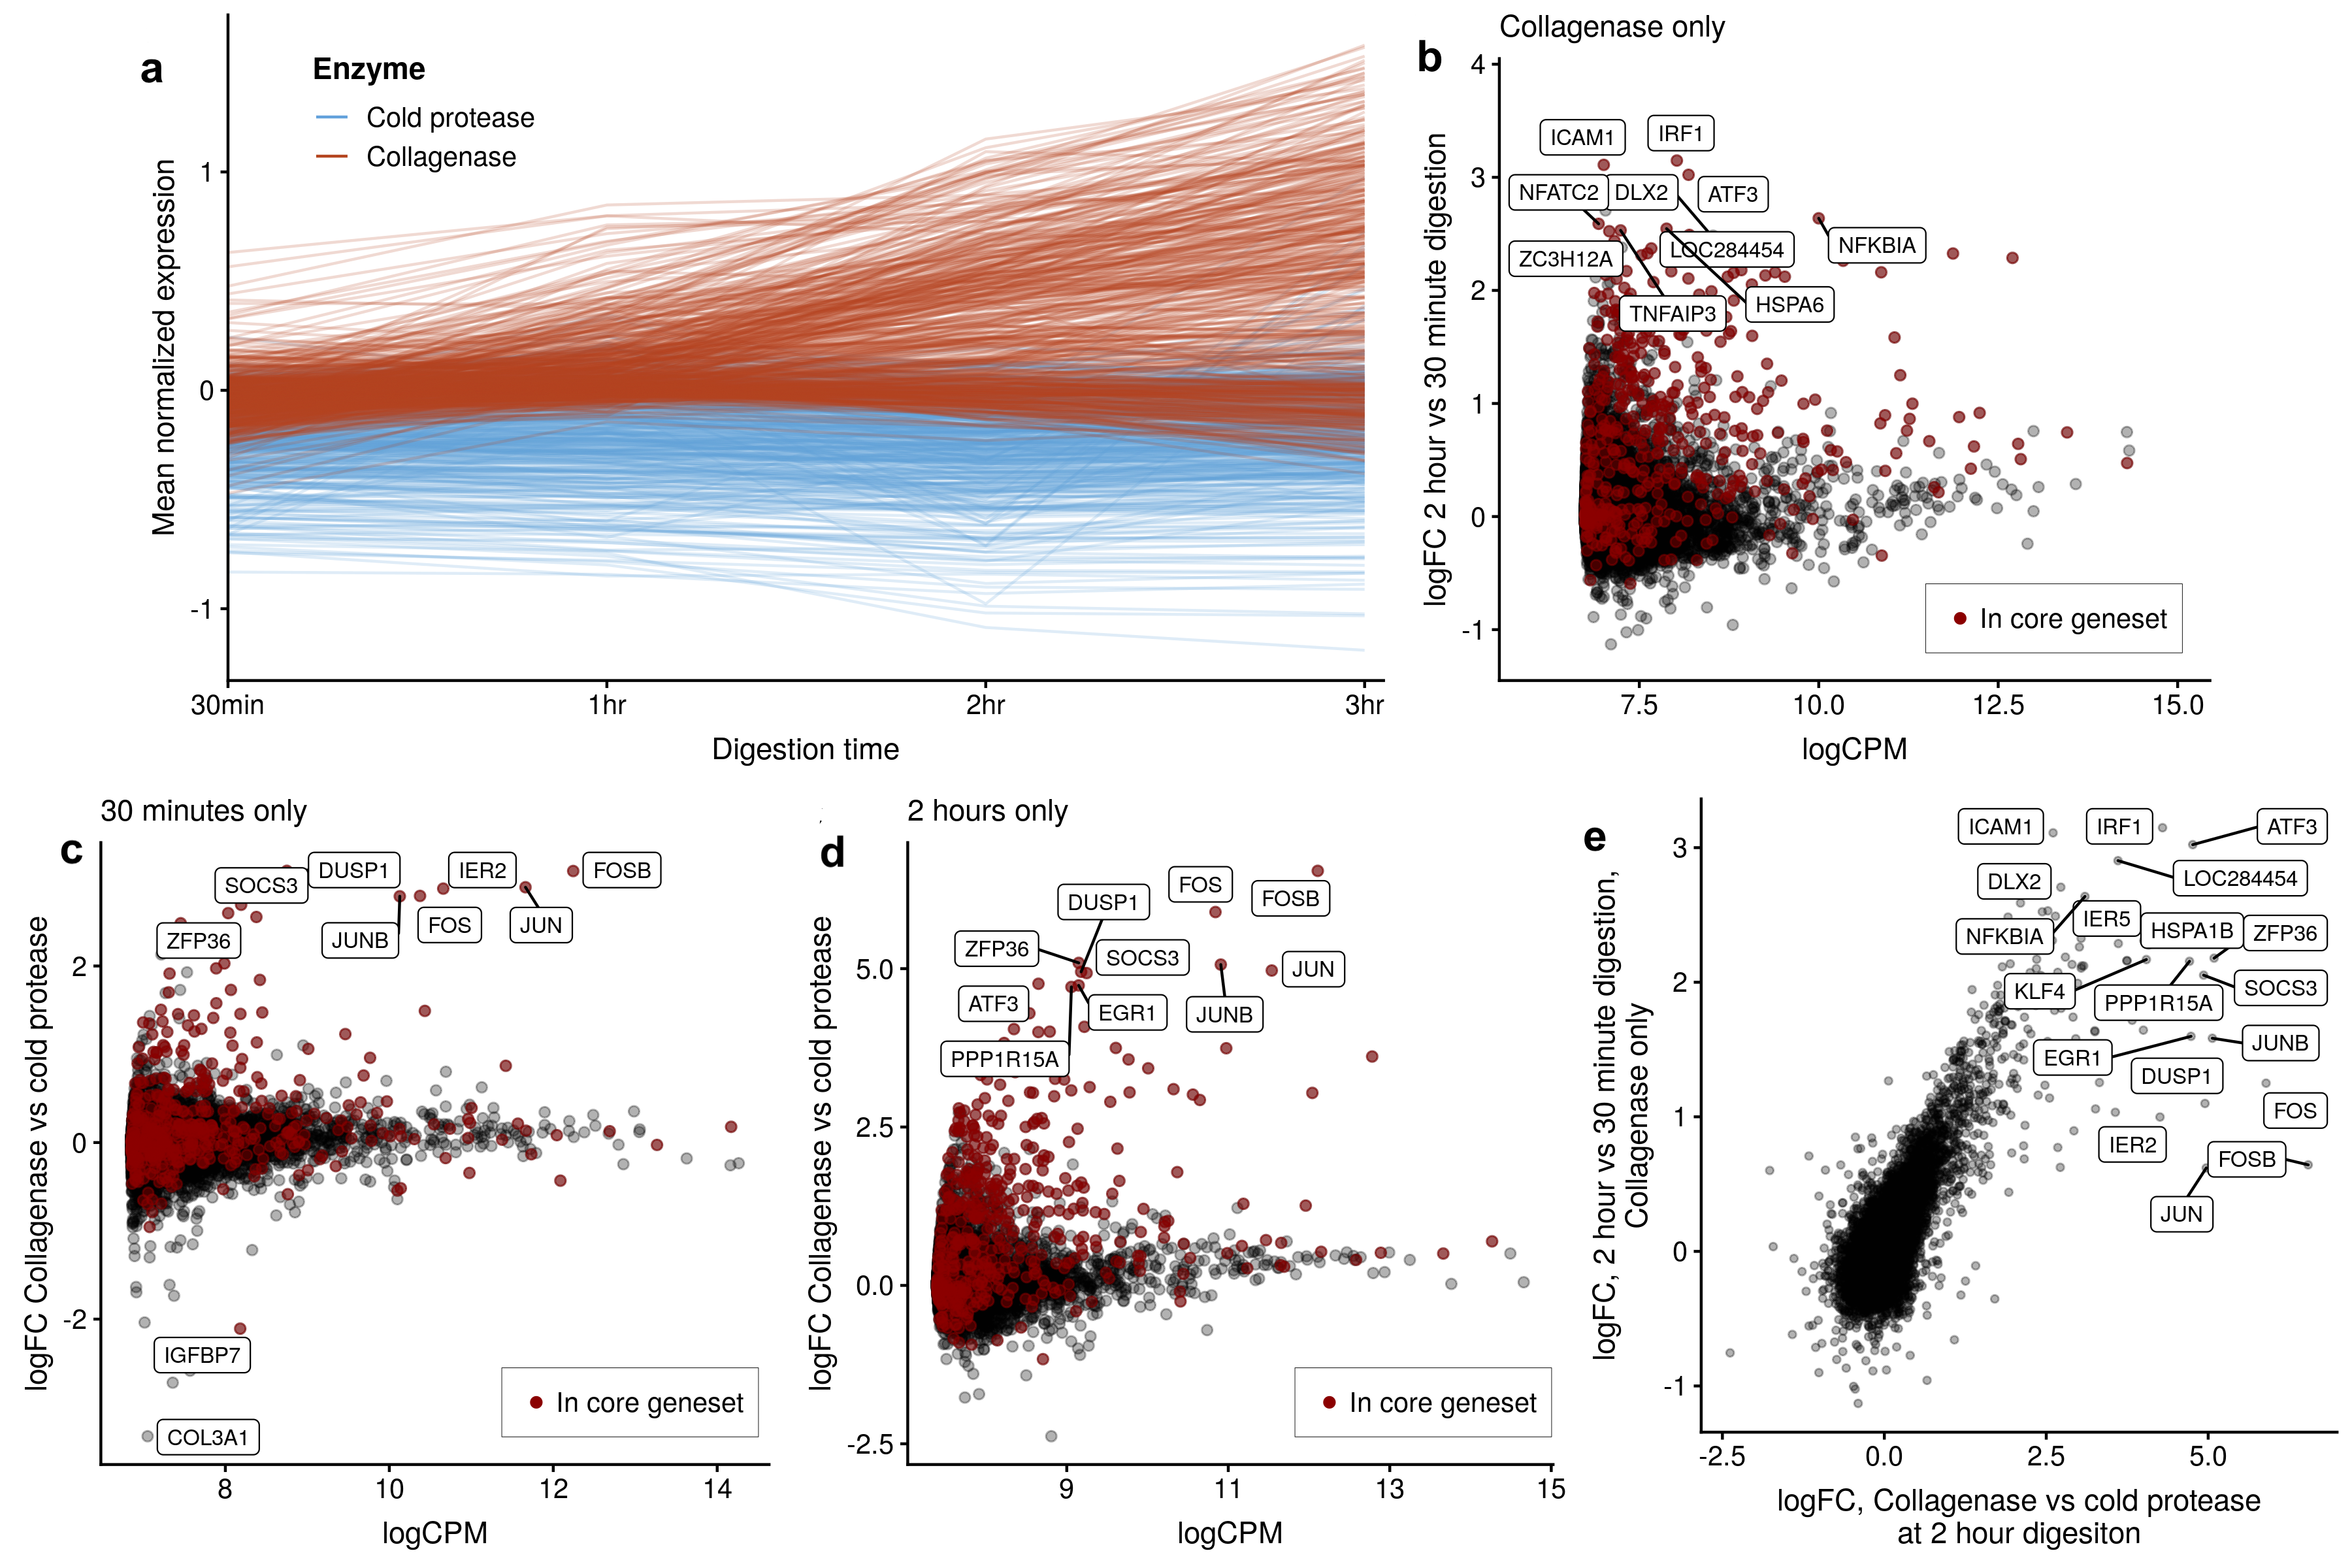
\includegraphics[width=\textwidth]{Figures/digestiontime.png}
	\caption[Differential expression of cluster 1 of live, dead, and dying cells.]
	{\small
	 \textbf{Disentangling the effects of digestion time and digestion method on transcriptomic response.}
    \textbf{(a)} Mean normalized expression of genes in the core gene set as a function of digestion time coloured by digestion temperature. Digestion by collagenase causes upregulation of the geneset at all timepoints, with a subset showing further upregulation as digestion time increases.
    \textbf{(b)} Log fold changes of a 2 hour vs. 30 minute digestion for collagenase only as a function of log counts-per-million. 
    \textbf{(c)} Log fold changes of a collagenase vs cold protease digestion at 30 minutes digestion time as a function of log counts-per-million. 
    \textbf{(d)} Log fold changes of a collagenase vs cold protease digestion at 2 hours digestion time as a function of log counts-per-million. 
    \textbf{(e)} The log fold changes of a 2 hour vs. 30 minute digestion (collageanse only) compared to a collagenase vs. cold protease digestion at 2 hours demonstrates a large overlap between genes affected ($\rho=$ 0.8).
    }
    \label{fig:time}
\end{figure}



Examining genes identified in the core gene set above, we found striking upregulation of the core gene set between collagenase and cold protease digestion at all digestion times \textbf{(Figure 3.8 a)}. This demonstrates that the choice of digestion enzyme (collagenase vs. cold protease) has an impact on the cells’ transcriptional response, independent of the length of digestion. However, a subset of the core gene set was further upregulated with increasing digestion time under collagenase digestion \textbf{(Figure 3.8 a)} . To quantify this, we performed several transcriptome-wide pairwise differential expression analyses to discern the effect of digestion conditions on transcriptomic response. Firstly, we compared a 30-min vs. 2 hours digestion using only collagenase \textbf{(Figure 3.8 b)} Of the 18,734 genes retained for differential expression analysis, 8,064 (43\%) were significantly differentially expressed ($<5\%$ FDR), with 4917 genes upregulated at 2h and 3,147 downregulated. Of the 512 genes in the core dissociation-associated gene set, 420 (82\%) were significantly differentially expressed (376 upregulated, 44 downregulated).
In contrast, repeating this analysis with cells digested using cold protease only revealed far fewer genes (2,500 of 16,340, 15.3\%) differentially expressed between the two digestion time points, with 35.9\% of the core gene set (70 upregulated, 114 downregulated) showing differential expression over time.
Secondly, we compared collagenase vs. cold protease digestion at 30 min only \textbf{(Figure 3.8 c)}. Of the 18,242 genes retained for differential expression analysis, 5039 (27.6\%) were significantly differentially expressed ($<5\%$ FDR), with 2,173 genes upregulated at 2 hours and 2,866 downregulated. Of the 512 genes in the core collagenase-associated gene set, 306 (59.8\%) were significantly differentially expressed (223 upregulated, 83 downregulated). Similarly, comparing collagenase vs. cold protease digestion at  2 hours only \textbf{(Figure 3.8 d)} found 7,887 of 17,345 genes (45.5\%) differentially expressed (4,207 upregulated, 3680 downregulated), with 429 of 512 (83.8\%) genes from the core gene set being differentially expressed (362 upregulated, 67 downregulated). These results robustly demonstrate that both digestion time and digestion method contribute to transcriptomic stress response in single cancer cells.
Interestingly, a highly similar set of genes are affected by both digestion time and digestion method, with a large correlation (Spearman’s $\rho=$ 0.8) between the log fold changes of contrasting 2-h to 30-min digestion (collagenase only) as compared to a collagenase vs. cold protease digestion at 30 min only \textbf{(Figure 3.8 e)}. These results suggest that the cellular response to digestion in single-cell transcriptomic experiments converge on a common set of pathways.


\section{Discussion}
In this chapter, we began with the intention of developing patient derived xenograft (PDX) in immunodeficient NOD Rag-1 null interleukin-2 receptor gamma null (NRG) and identifying the dose response properties of PDX to determine relative ability of the drugs to produce maximum functional response.

To establish PDX models, patient-derived tumors need to be injected into highly immunodeficient mice, because the mouse immune system could eradicate transplanted cancer cells and prohibit tumor engraftment. Developing models that mimic human cancer is a long-standing goal in cancer research \cite{aparicio2015examining, may2018cancer, ryu2019integrative}. In order to reach to final formation of longitudinal chemotherapy perturbed model systems, it was important to successfully create PDX in immunodeficient NOD Rag-1 null interleukin-2 receptor gamma null (NRG) instead of highly immunodeficient NOD/SCID/IL2rγ−/− (NSG). It is by now well known that NRG mice can harbor established PDX, and can tolerate aggressive induction chemotherapy at higher doses than NSG mice without overt toxicity \cite{barve2018comparative}. 

Next important step was to select breast PDX and the chemotherapies that could be used in cancer evolution studies. SA609, SA1035 and SA535 tend to show high sensitivity for platinum so these were selected for making a timeseries model for the next chapter 4. CX-5461, G4 stabilizer drug showed synthetic lethality with DNA repair pathway deficiency in \textit{in vitro} cultures as \cite{xu2017cx}, so along with treating for timeseries with cisplatin, we selected SA535 (BRCA1-HRD) for CX-5461 in parallel for timeseries drug perturbation for the next chapter.

Recent advancements in sequencing technologies have allowed for DNA and RNA sequencing at single-cell resolution, which can be used to interrogate genomes and transcriptomes of tumor tissues that may not be resolved by bulk sequencing, such as intratumoral heterogeneity, clonal dynamics, and the mapping of known and de novo cell types.However, various steps can impact the quality and quantity of these single cells for sequencing analysis.
Here we sought to optimize conditions and factors that could participate single cell sequencing outcome. Standard sample preparation methods for solid tissues require enzymatic and mechanical dissociation and, depending on the tissue origin, density, disease state, elastin, or collagen content, may require long enzymatic digestion and/or vigorous mechanical disruption.
For single cell whole genome sequencing the additional step of dead cell removal from the final single cell suspension tend to show  cleaner cells, less debris and high percent viability providing high chances of live cells taken up by the robotic spotters as explained in \cite{laks2019clonal}. 

Current sequencing techniques require single-cell suspensions for passage through microfluidic or microwell platforms, and the generation of single-cell suspensions from solid tissues requires the enzymatic and mechanical disruption of extracellular matrix and cell-cell contacts. To date, the effect of these dissociation methods on the transcriptome of single cells has been largely ignored, despite the potential effects on the interpretation of scRNA-seq data. Moreover, during both dissociation of tissues and passage through fluidic devices, cells can undergo stress, shearing, anoikis, and apoptosis \cite{aljanahi2018introduction}. For this reason, efforts must be made on both sample handling and bioinformatics to ensure minimal noise and optimal filtration of data. Here, we endeavored to describe the artifactual gene expression associated with tissue dissociation and dead or dying cell populations. Using a large, diverse dataset, we highlight the variability in key QC metrics, including the percentage of mitochondrial genes, number of UMIs, and number of genes detected. 

We identify sub-populations of dead cells that express either high or low mitochondrial genes, contrary to the notion that dead cells can be characterized by their mitochondrial gene content alone. Importantly, cells that are FACS sorted as either live, dying, or dead based on PI/annexin V staining are present in all three clusters, highlighting that the transcriptomic state of the cell is not necessarily the same as the surface marker state (though the two are correlated). As noted, this is reminiscent of “pseudotime” orderings, with PC1 from \textbf{Figure 3.6 a} approximating a trajectory through the data that tracks transcriptomically healthy cells to transcriptomically dead cells with increasing PC1 values. Though expressing transcriptomes similar to live, healthy cells, dead cells with low mitochondrial content expressed significantly high levels of MHC class I genes such as HLA-A, HLA-B, and B2M.

 We identified a sub-population of dead cells that would not be removed through standard data filtering practices and quantify the extent to which their transcriptomes differ from live sorted cells. We identified a further sub-population that represents transcriptomically dying cells, expressing increased major histocompatibility complex (MHC)-class I genes. We also identified a core gene set of immediate, heat shock, and stress response genes associated with collagenase dissociation, highly conserved across cell and tissue types, and which are minimized by dissociation at cold temperature.






